% Options for packages loaded elsewhere
\PassOptionsToPackage{unicode}{hyperref}
\PassOptionsToPackage{hyphens}{url}
\PassOptionsToPackage{dvipsnames,svgnames,x11names}{xcolor}
%
\documentclass[
  letterpaper,
  DIV=11,
  numbers=noendperiod]{scrreprt}

\usepackage{amsmath,amssymb}
\usepackage{iftex}
\ifPDFTeX
  \usepackage[T1]{fontenc}
  \usepackage[utf8]{inputenc}
  \usepackage{textcomp} % provide euro and other symbols
\else % if luatex or xetex
  \usepackage{unicode-math}
  \defaultfontfeatures{Scale=MatchLowercase}
  \defaultfontfeatures[\rmfamily]{Ligatures=TeX,Scale=1}
\fi
\usepackage{lmodern}
\ifPDFTeX\else  
    % xetex/luatex font selection
\fi
% Use upquote if available, for straight quotes in verbatim environments
\IfFileExists{upquote.sty}{\usepackage{upquote}}{}
\IfFileExists{microtype.sty}{% use microtype if available
  \usepackage[]{microtype}
  \UseMicrotypeSet[protrusion]{basicmath} % disable protrusion for tt fonts
}{}
\makeatletter
\@ifundefined{KOMAClassName}{% if non-KOMA class
  \IfFileExists{parskip.sty}{%
    \usepackage{parskip}
  }{% else
    \setlength{\parindent}{0pt}
    \setlength{\parskip}{6pt plus 2pt minus 1pt}}
}{% if KOMA class
  \KOMAoptions{parskip=half}}
\makeatother
\usepackage{xcolor}
\setlength{\emergencystretch}{3em} % prevent overfull lines
\setcounter{secnumdepth}{5}
% Make \paragraph and \subparagraph free-standing
\ifx\paragraph\undefined\else
  \let\oldparagraph\paragraph
  \renewcommand{\paragraph}[1]{\oldparagraph{#1}\mbox{}}
\fi
\ifx\subparagraph\undefined\else
  \let\oldsubparagraph\subparagraph
  \renewcommand{\subparagraph}[1]{\oldsubparagraph{#1}\mbox{}}
\fi


\providecommand{\tightlist}{%
  \setlength{\itemsep}{0pt}\setlength{\parskip}{0pt}}\usepackage{longtable,booktabs,array}
\usepackage{calc} % for calculating minipage widths
% Correct order of tables after \paragraph or \subparagraph
\usepackage{etoolbox}
\makeatletter
\patchcmd\longtable{\par}{\if@noskipsec\mbox{}\fi\par}{}{}
\makeatother
% Allow footnotes in longtable head/foot
\IfFileExists{footnotehyper.sty}{\usepackage{footnotehyper}}{\usepackage{footnote}}
\makesavenoteenv{longtable}
\usepackage{graphicx}
\makeatletter
\def\maxwidth{\ifdim\Gin@nat@width>\linewidth\linewidth\else\Gin@nat@width\fi}
\def\maxheight{\ifdim\Gin@nat@height>\textheight\textheight\else\Gin@nat@height\fi}
\makeatother
% Scale images if necessary, so that they will not overflow the page
% margins by default, and it is still possible to overwrite the defaults
% using explicit options in \includegraphics[width, height, ...]{}
\setkeys{Gin}{width=\maxwidth,height=\maxheight,keepaspectratio}
% Set default figure placement to htbp
\makeatletter
\def\fps@figure{htbp}
\makeatother
% definitions for citeproc citations
\NewDocumentCommand\citeproctext{}{}
\NewDocumentCommand\citeproc{mm}{%
  \begingroup\def\citeproctext{#2}\cite{#1}\endgroup}
\makeatletter
 % allow citations to break across lines
 \let\@cite@ofmt\@firstofone
 % avoid brackets around text for \cite:
 \def\@biblabel#1{}
 \def\@cite#1#2{{#1\if@tempswa , #2\fi}}
\makeatother
\newlength{\cslhangindent}
\setlength{\cslhangindent}{1.5em}
\newlength{\csllabelwidth}
\setlength{\csllabelwidth}{3em}
\newenvironment{CSLReferences}[2] % #1 hanging-indent, #2 entry-spacing
 {\begin{list}{}{%
  \setlength{\itemindent}{0pt}
  \setlength{\leftmargin}{0pt}
  \setlength{\parsep}{0pt}
  % turn on hanging indent if param 1 is 1
  \ifodd #1
   \setlength{\leftmargin}{\cslhangindent}
   \setlength{\itemindent}{-1\cslhangindent}
  \fi
  % set entry spacing
  \setlength{\itemsep}{#2\baselineskip}}}
 {\end{list}}
\usepackage{calc}
\newcommand{\CSLBlock}[1]{\hfill\break\parbox[t]{\linewidth}{\strut\ignorespaces#1\strut}}
\newcommand{\CSLLeftMargin}[1]{\parbox[t]{\csllabelwidth}{\strut#1\strut}}
\newcommand{\CSLRightInline}[1]{\parbox[t]{\linewidth - \csllabelwidth}{\strut#1\strut}}
\newcommand{\CSLIndent}[1]{\hspace{\cslhangindent}#1}

\KOMAoption{captions}{tableheading}
\makeatletter
\@ifpackageloaded{tcolorbox}{}{\usepackage[skins,breakable]{tcolorbox}}
\@ifpackageloaded{fontawesome5}{}{\usepackage{fontawesome5}}
\definecolor{quarto-callout-color}{HTML}{909090}
\definecolor{quarto-callout-note-color}{HTML}{0758E5}
\definecolor{quarto-callout-important-color}{HTML}{CC1914}
\definecolor{quarto-callout-warning-color}{HTML}{EB9113}
\definecolor{quarto-callout-tip-color}{HTML}{00A047}
\definecolor{quarto-callout-caution-color}{HTML}{FC5300}
\definecolor{quarto-callout-color-frame}{HTML}{acacac}
\definecolor{quarto-callout-note-color-frame}{HTML}{4582ec}
\definecolor{quarto-callout-important-color-frame}{HTML}{d9534f}
\definecolor{quarto-callout-warning-color-frame}{HTML}{f0ad4e}
\definecolor{quarto-callout-tip-color-frame}{HTML}{02b875}
\definecolor{quarto-callout-caution-color-frame}{HTML}{fd7e14}
\makeatother
\makeatletter
\@ifpackageloaded{bookmark}{}{\usepackage{bookmark}}
\makeatother
\makeatletter
\@ifpackageloaded{caption}{}{\usepackage{caption}}
\AtBeginDocument{%
\ifdefined\contentsname
  \renewcommand*\contentsname{Tabla de contenidos}
\else
  \newcommand\contentsname{Tabla de contenidos}
\fi
\ifdefined\listfigurename
  \renewcommand*\listfigurename{Listado de Figuras}
\else
  \newcommand\listfigurename{Listado de Figuras}
\fi
\ifdefined\listtablename
  \renewcommand*\listtablename{Listado de Tablas}
\else
  \newcommand\listtablename{Listado de Tablas}
\fi
\ifdefined\figurename
  \renewcommand*\figurename{Figura}
\else
  \newcommand\figurename{Figura}
\fi
\ifdefined\tablename
  \renewcommand*\tablename{Tabla}
\else
  \newcommand\tablename{Tabla}
\fi
}
\@ifpackageloaded{float}{}{\usepackage{float}}
\floatstyle{ruled}
\@ifundefined{c@chapter}{\newfloat{codelisting}{h}{lop}}{\newfloat{codelisting}{h}{lop}[chapter]}
\floatname{codelisting}{Listado}
\newcommand*\listoflistings{\listof{codelisting}{Listado de Listados}}
\makeatother
\makeatletter
\makeatother
\makeatletter
\@ifpackageloaded{caption}{}{\usepackage{caption}}
\@ifpackageloaded{subcaption}{}{\usepackage{subcaption}}
\makeatother
\ifLuaTeX
\usepackage[bidi=basic]{babel}
\else
\usepackage[bidi=default]{babel}
\fi
\babelprovide[main,import]{spanish}
% get rid of language-specific shorthands (see #6817):
\let\LanguageShortHands\languageshorthands
\def\languageshorthands#1{}
\ifLuaTeX
  \usepackage{selnolig}  % disable illegal ligatures
\fi
\usepackage{bookmark}

\IfFileExists{xurl.sty}{\usepackage{xurl}}{} % add URL line breaks if available
\urlstyle{same} % disable monospaced font for URLs
\hypersetup{
  pdftitle={Bitácora Grupo 3 , CA-204 (II-2024)},
  pdfauthor={Joseph Romero, Cristhofer Urrutia, Oscar Espinoza},
  pdflang={es},
  colorlinks=true,
  linkcolor={blue},
  filecolor={Maroon},
  citecolor={Blue},
  urlcolor={Blue},
  pdfcreator={LaTeX via pandoc}}

\title{Bitácora Grupo 3 , CA-204 (II-2024)}
\author{Joseph Romero, Cristhofer Urrutia, Oscar Espinoza}
\date{2024-09-28}

\begin{document}
\maketitle

\renewcommand*\contentsname{Tabla de contenidos}
{
\hypersetup{linkcolor=}
\setcounter{tocdepth}{2}
\tableofcontents
}
\bookmarksetup{startatroot}

\chapter*{Introducción}\label{introducciuxf3n}
\addcontentsline{toc}{chapter}{Introducción}

\markboth{Introducción}{Introducción}

En este proyecto se investigará qué características hacen que los
videojuegos sean preferidos por los consumidores, para esto se utilizará
una base de datos que contiene información sobre diferentes videojuegos
y sus atributos. Lo que se quiere conseguir con lo anterior es descubrir
patrones y relaciones que ayuden a entender qué elementos son clave para
que un videojuego sea preferido por sobre los demás y para lograr esto
se aplicarán técnicas de análisis de datos, para así poder identificar
las características que hacen a esos juegos exitosos.

\bookmarksetup{startatroot}

\chapter{Bitácora 1}\label{bituxe1cora-1}

\section{Comando 1:}\label{comando-1}

\begin{figure}[H]

{\centering 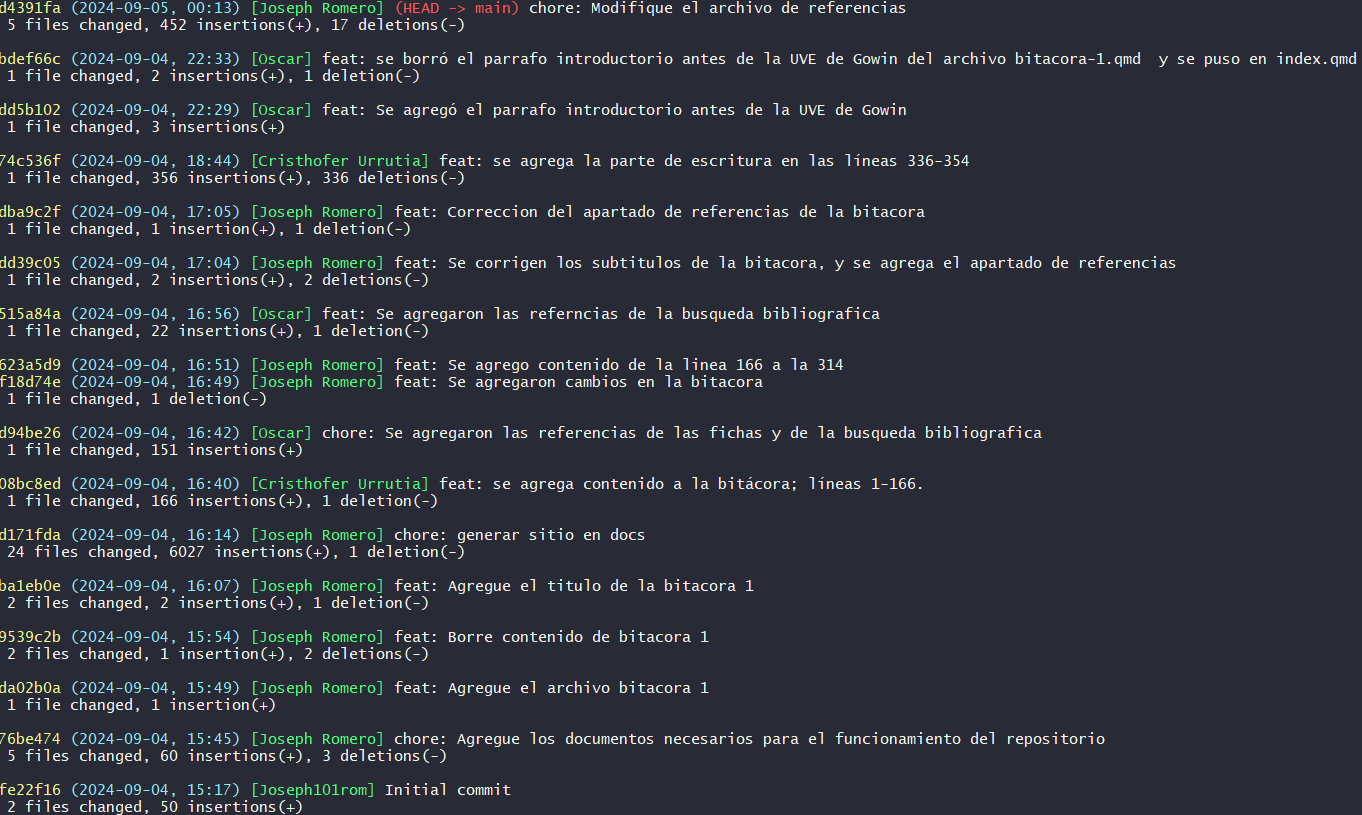
\includegraphics{imagenes/link-1.png}

}

\caption{Resultado del link}

\end{figure}%

\section{Comando 2:}\label{comando-2}

\begin{figure}[H]

{\centering 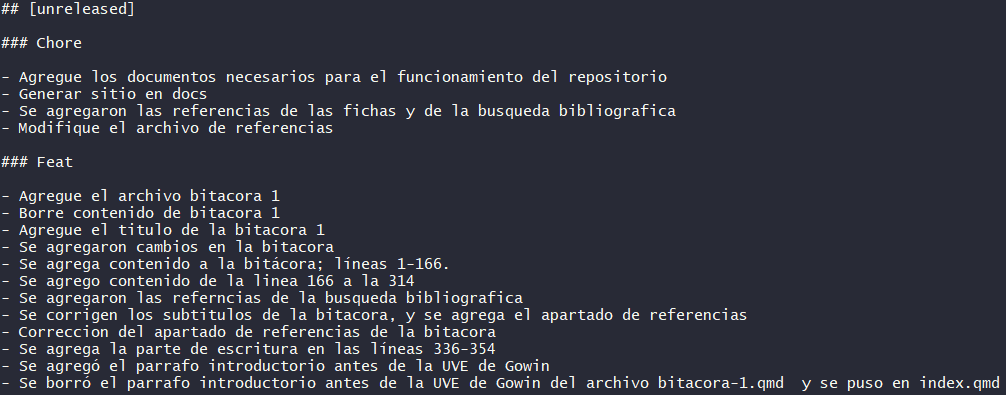
\includegraphics{imagenes/CHANGELOG-1.png}

}

\caption{Changelog}

\end{figure}%

\section{Comando 3:}\label{comando-3}

\begin{figure}[H]

{\centering 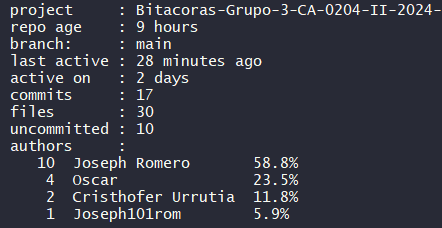
\includegraphics{imagenes/gitsummary-1.png}

}

\caption{Git summary}

\end{figure}%

\bookmarksetup{startatroot}

\chapter{Parte planificacion}\label{parte-planificacion}

\section{Pregunta de investigación:}\label{pregunta-de-investigaciuxf3n}

\subsection{Defincion del idea}\label{defincion-del-idea}

``Análisis del Éxito Comercial de Videojuegos Basado en Características
del Juego''

\subsection{Conceptualización de la
idea:}\label{conceptualizaciuxf3n-de-la-idea}

\begin{itemize}
\item
  Análisis: Por análisis se entiende el examen minucioso y pormenorizado
  de un asunto para conocer su naturaleza, sus características, su
  estado y los factores que intervienen en todo ello.
  \href{https://definicion.edu.lat/significados/analisis.html\#:~:text=Qu\%C3\%A9\%20es\%20An\%C3\%A1lisis\%3A\%20Por\%20an\%C3\%A1lisis\%20se\%20entiende\%20el,y\%20los\%20factores\%20que\%20intervienen\%20en\%20todo\%20ello.}{Fuente}
\item
  Éxito: El éxito es el resultado satisfactorio de una acción o
  proyecto.
  \href{https://definicion.edu.lat/concepto/exito.html}{Fuente}
\item
  Comercial: Comercial es un adjetivo que se refiere a lo vinculado con
  el comercio o con las personas que se dedican a comprar y/o vender
  bienes o servicios. El término comercio, por su parte, puede hacer
  mención a esta actividad o al espacio físico donde se desarrolla.
  \href{https://definicion.edu.lat/definicion/comercial.html}{Fuente}
\item
  Videojuegos: Los videojuegos son softwares de juegos electrónicos
  desarrollados para el entretenimiento a través de un aparato
  electrónico como máquinas arcade, consolas, computadores o
  dispositivos digitales.
  \href{https://definicion.edu.lat/significados/videojuego.html}{Fuente}
\item
  Basado: La palabra ``basado'' es el participio del verbo ``basar'' y
  se utiliza como un adjetivo para describir algo que se ha fundamentado
  o apoyado en una base específica.
  \href{https://www.definiciones-de.com/Definicion/de/basado.php\#:~:text=Definici\%C3\%B3n\%20de\%20basado\%20p.\%20La\%20palabra\%20\%22basado\%22\%20es,base\%20determinada\%2C\%20sin\%20perder\%20completamente\%20su\%20naturaleza\%20verbal.}{Fuente}
\item
  Característica: Las características de un objeto, una persona o un
  referente cualquiera son aquellos rasgos, condiciones o elementos que
  le resultan propios, reconocibles y que sirven para distinguirlo de
  otros referentes similares. Así, por ejemplo, las características de
  un perro incluyen su color, su tamaño, su raza, su conducta, su edad y
  todo aquello que nos sirva para distinguirlo del resto de los
  animales.
  \href{https://definicion.edu.lat/concepto/caracteristica.html}{Fuente}
\item
  Juego: Ejercicio recreativo o de competición sometido a reglas, y en
  el cual se gana o se pierde. \href{https://dle.rae.es/juego}{Fuente}
\end{itemize}

\subsection{Identificación de
tensiones:}\label{identificaciuxf3n-de-tensiones}

Definición de Variables y Métricas: Consideramos fundamental definir
correctamente las variables y las métricas de manera clara y concisa, ya
que en caso de no hacerlo puede resultar en una labor mucho más extensa
y complicada de lo esperado.

Selección de Técnicas de Análisis: En caso de no realizar una correcta
selección de técnicas de análisis, podríamos enfrentarnos ante un
proceso más largo y complicado de lo que debería de ser, además de no
brindar información fidedigna al analizar los datos con una técnica
inadecuada.

Definición de ``Éxito Comercial'': Pensamos que establecer una métrica
clara y consistente para medir el éxito comercial de los videojuegos
puede representar todo un desafío, pues este es un concepto que puede
depender de factores como ventas, popularidad e ingresos, lo que lo
vuelve un poco más complicado el ``limitar'' a la hora de definirlo.

Identificación de Características Clave del Juego: En caso de no escoger
las características de videojuegos adecuadas, puede que estas no estén
presentes en nuestra base de datos o que no nos lleven a conclusiones
relevantes, por ende afectando la integridad del proyecto.

Complejidad de las Relaciones: Entender las relaciones que pueden o no
darse entre las características del juego y el éxito comercial puede ser
algo complicado, pues existen interacciones y efectos que no son
precisamente lineales y que podrían requerir de técnicas de análisis
avanzadas (de las cuales no disponemos en este curso), lo que añade una
capa más de complejidad a nuestro estudio que no fué contemplada al
inicio.

Comparabilidad entre Juegos: Los videojuegos pueden diferir
significativamente en términos de presupuesto, marketing y otros
factores externos al juego en sí, lo cual puede hacer más difícil aislar
el efecto de las características de cada juego en el éxito comercial y
por ende dificultarnos la labor de llegar a concluir alguna relación
entre el juego y las características que lo llevaron ser exitoso.

\subsection{Reformulación de la idea en modo
pregunta}\label{reformulaciuxf3n-de-la-idea-en-modo-pregunta}

\begin{itemize}
\item
  ¿Cómo se puede analizar el mercado de los videojuegos?
\item
  ¿Por qué es importante analizar el mercado de los videojuegos para
  reconocer desencadenantes del éxito de la industria?
\item
  ¿Qué características son fundamentales para el éxito comercial de un
  videojuego dado el contexto donde fue publicado?
\item
  ¿Por qué a las personas les atraen los videojuegos y cuál es su
  relación con el éxito comercial de los videojuegos?
\end{itemize}

\subsection{Argumentación de la
preguntas:}\label{argumentaciuxf3n-de-la-preguntas}

¿Cómo se puede analizar el mercado de los videojuegos?

\emph{Contrargumentos:}

\begin{itemize}
\item
  \emph{Lógica:} El análisis podría ser limitado si se considerara un
  subanálisis predictivo. Esto debido a que el mercado puede dar giros
  radicales; por ejemplo, se puede dar el caso de que anuncien una nueva
  consola de videojuegos.
\item
  \emph{Ética:} Existen videojuegos cuya temática es la violencia y
  realizar un proyecto donde se mencionan dichos videojuegos podría
  conducir a una publicidad accidental de un mercado de juegos
  violentos.
\item
  \emph{Emocional:} Un análisis simplificado del mercado de los
  videojuegos puede omitir aspectos como la propia perspectiva de un
  consumidor frente a cierto tipo de videojuegos, por ejemplo.
\end{itemize}

\emph{Argumentos:}

\begin{itemize}
\item
  \emph{Lógica:} El análisis de este mercado podría aprovecharse de
  herramientas microeconómicas y macroeconómicas, pues a fin de cuentas
  sigue siguiendo un mercado.
\item
  \emph{Ética:} La mayoría de videojuegos requieren conexión permanente
  a internet, además, plataformas de videojuegos oficiales como Steam
  permiten acceder a bases de datos sobre videojugadores. Por lo tanto
  la información obtenida probablemente esté inalterada.
\item
  \emph{Emocional:} Gracias a los datos se podría ver que tan rentable
  es la industria de los videojuegos y de esta manera informar a la
  gente sobre dicha conclusión, pues existen muchas personas
  desempleadas que podrían incorporarse al mercado.
\end{itemize}

\emph{Conclusión:} El mercado de los videojuegos, como cualquier otro,
presenta sus propias problemáticas micro y macroeconómicas. Es gracias a
la salvedad de las herramientas económicas que se podrá hacer un
análisis desde ambas perspectivas (consumidor y empresas), sin embargo
se tendría un rezago en la parte emocional de las preferencias, por lo
que el análisis puede llegar a ser considerado tosco.

¿Por qué es importante analizar el mercado de los videojuegos para
reconocer desencadenantes del éxito de la industria?

\emph{Contrargumentos:}

\begin{itemize}
\item
  \emph{Lógica:} Existen otros mercados cuya influencia trasciende
  sustancialmente al de los videojuegos, un ejemplo de estos mercados
  puede ser el del petróleo, pues muchas actividades del día a día
  dependen de dicho recurso.
\item
  \emph{Ética:} En los últimos años se ha generado una gran ola de
  denuncias por parte de los trabajadores hacía las compañías
  desarrolladoras de videojuegos, lamentablemente, existen países como
  Japón en donde por su cultura los trabajadores no suelen visibilizar
  las problemáticas en los ambientes laborales. Por esta razón, la
  importancia de analizar este mercado no podría estar tan bien
  conceptualizada en este tipo de países. También podría darse el caso
  de que ciertos datos estén mostrando información ``falsa'', pues si se
  quisiera analizar las horas jugadas por jugador para asociar esto con
  las ventas, habría que tener en cuenta que muchas de esas horas
  corresponden a gente que estaba \emph{afk}.
\item
  \emph{Emocional:} La preferencia de los consumidores estarían
  respaldadas bajo datos estadísticos; lo que implica que se ignorarán
  experiencias que los jugadores hayan experimentado mientras jugaban.
\end{itemize}

\emph{Argumentos:}

\begin{itemize}
\item
  \emph{Lógica:} A nivel cultural sería interesante sonsacar la
  importancia de este mercado. Como expresión artística, los videojuegos
  podrían indicar una respuesta social a ciertos fenómenos de la
  actualidad como ha pasado con la música. Los datos estadísticos
  ayudarían a esclarecer este suceso.
\item
  \emph{Ética:} Un país en desarrollo como Costa Rica podría tomar
  acción al incursionar (o no) en el mercado de videojuegos gracias a
  las estadísticas. Si un país lograra éxito en este mercado sería
  posible aumentar las fuentes de ingresos.
\item
  \emph{Emocional:} Para muchas personas los videojuegos se les
  presentaron en su infancia; sería de especial interés conocer qué
  empresas han permanecido con sus sagas longevas de videojuegos y de
  esta manera complacer a sus consumidores.
\end{itemize}

\emph{Conclusión:} Pese a que bajo ciertas medidas los videojuegos no
sean una industria tan influyente, siempre existirá este mercado de
nicho que se mueve principalmente por razones emocionales. También es
importante recalcar irregularidades del mercado para que se puedan
corregir en el futuro y de esta manera mejorar el ambiente laboral, por
ejemplo. También, aunque parezca utópico por la naturaleza del tema: el
análisis puede servir para que gobiernos decidan si invertir recursos en
la industria.

¿Qué características son fundamentales para el éxito comercial de un
videojuego dado el contexto donde fue publicado?

\emph{Contrargumentos:}

\begin{itemize}
\item
  \emph{Lógica}: Los resultados de este análisis podrían no ser
  concretos. Los videojuegos empezaron a ser más notorios en la década
  de los 70 y desde entonces las tendencias han cambiado radicalmente.
\item
  \emph{Ética:} Si se fija el análisis dentro de un período específico,
  se obtendrían datos sobre características propias de videojuegos
  violentos, un ejemplo de esto es la década 2010-2020. De esta manera,
  se puede dar el caso de que algún grupo de personas interpreten de
  manera errónea la información.
\item
  \emph{Emocional:} Existen datos no parametrizables que pueden
  determinar el éxito de un videojuego, por ejemplo: la relación que
  pueden entablar varias personas en los juegos en línea.
\end{itemize}

\emph{Argumentos:}

\begin{itemize}
\item
  \emph{Lógica:} Sería posible tener un análisis que demuestre el
  panorama actual de las preferencias de los videojugadores, por lo que
  a nivel sociológico o cultural se podrían notar patrones en las
  características de los videojuegos. Por ejemplo, una característica
  que sería de gran ayuda para este propósito es la de ``géneros de los
  videojuegos''.
\item
  \emph{Ética:} Gracias a las características notadas, se podrían
  realizar sugerencias acerca de cómo tendrían que ser los videojuegos
  para mantener al público satisfecho.
\item
  \emph{Emocional:} El nicho de los videojuegos tiene una característica
  muy importante: la sociabilidad entre sus miembros. Realizar este
  análisis permitiría que las personas conozcan más acerca de sus
  preferencias en videojuegos y se vean incentivadas a socializar más.
\end{itemize}

\emph{Conclusión:} Aunque las características sean cambiantes, vale la
pena realizar un análisis sobre períodos fijos y de esta manera conocer
cuáles características fueron prevalecientes en dichos períodos. Un
punto bueno de este análisis es el de la posibilidad de notar las
mejores características de cada época y combinarlas para tratar de
combatir irregularidades del presente.

¿Por qué a las personas les atraen los videojuegos y su relación con el
éxito de la industria?

\emph{Contraargumentos:}

\begin{itemize}
\item
  \emph{Lógica:} Esta pregunta tiene una fuerte connotación emocional.
  Por lo tanto, resulta difícil socavar la premisa mediante datos
  numéricos y categóricos sencillos.
\item
  \emph{Ética:} Se ha visto casos de criminales que usan como medio a
  los videojuegos para realizar sus actos infames. Esto sucede gracias a
  juegos en línea en donde por ejemplo, un extorsionador puede utilizar
  a un infante para sus propósitos, por este y muchos otros motivos los
  videojuegos son atractivos para la delincuencia y los datos serían
  imprecisos para notarlo.
\item
  \emph{Emocional:} La atracción a los videojuegos puede conducir a una
  posterior adicción a los videojuegos, lo que repercute en
  consecuencias sociales negativas para el ya paciente psiquiátrico
  afectado. Desgraciadamente, la incorporación de este trastorno al
  DSM-V fue reciente por lo que no se tienen suficientes datos de este
  tema.
\end{itemize}

\emph{Argumentos:}

\begin{itemize}
\item
  \emph{Lógica:} No podemos hablar de éxito de los videojuegos (a un
  nivel más profundo) basados en sus características sin antes responder
  a esta interrogante, pues es de la respuesta que obtenemos en una
  versión más primitiva (pero al mismo tiempo madura) una lista de las
  tan ansiadas características asociadas a dicho éxito desde el punto de
  vista del videojugador.
\item
  \emph{Ética:} Es menester de la sociedad conocer a través de un
  análisis los patrones de conducta que llevaron al auge y vigencia este
  fenómeno. De este modo la población en general tendrá un mejor juicio
  y panorama acerca del tema.
\item
  \emph{Emocional:} Un mundo sin videojuegos sería inimaginable para
  muchas personas, al final de cuentas muchas personas utilizan a los
  videojuegos como una herramienta para escapar de su realidad. Conocer
  qué factores están anudados a esta ``fuga'' de realidad podría ayudar
  a las personas a buscar ayuda psicológica y/o mejorarla.
\end{itemize}

\emph{Conclusión:} El punto más débil es la falta de información que
pueden tener ciertos indicadores numéricos y categóricos para abstraer
esta pregunta y responder. Sin embargo, se podría solventar ese problema
al investigar de manera un poco más profunda sobre la conducta humana y
estadísticas que se usen en estudios con propósito similar.

\subsection{Argumentacion a traves de
datos.}\label{argumentacion-a-traves-de-datos.}

\emph{Fuente de Información:} La base de datos utilizada es el Steam
Games Dataset, recopilado por Martin Bustos Roman en 2022 y disponible
en Kaggle. Este dataset incluye información detallada sobre más de
85,000 videojuegos publicados en la plataforma Steam. El enlace de
acceso es: https://doi.org/10.34740/KAGGLE/DS/2109585.

\emph{Contexto Temporal y Espacial de los Datos:} Temporal: El dataset
cubre videojuegos lanzados desde los inicios de Steam hasta el año 2022,
lo que permite analizar la evolución del mercado de videojuegos durante
un período largo. Espacial: El dataset abarca un contexto espacial
mundial, lo que permite realizar análisis que reflejen las tendencias y
características del mercado de videojuegos a nivel internacional.

\emph{Facilidad de Obtener la Información:} La base de datos es de
acceso público a través de Kaggle, lo que facilita la obtención y uso de
la información. La recopilación de datos fue realizada utilizando la API
de Steam, complementada con datos de Steam Spy.

\emph{Población de Estudio:} La población de estudio incluye todos los
videojuegos disponibles en Steam, lo que representa una cobertura
extensa del mercado de videojuegos .

\emph{Muestra Observada:} La muestra observada consta de más de 85,000
videojuegos, proporcionando una base sólida y representativa para el
análisis.

\emph{Unidad Estadística o Individuos:} Cada unidad estadística en la
tabla representa un videojuego individual. Cada fila en la tabla
corresponde a un juego específico con sus características particulares,
como precio, fecha de lanzamiento, reseñas, entre otros.

\textbf{Descripción de las Variables de la Tabla}

\begin{itemize}
\tightlist
\item
  \textbf{AppID:} Identificador único del juego en Steam.
\item
  \textbf{Name:} Nombre del juego.
\item
  \textbf{Release date:} Fecha de lanzamiento del juego.
\item
  \textbf{Estimated owners:} Número estimado de propietarios del juego.
\item
  \textbf{Peak CCU:} Máximo número de usuarios concurrentes.
\item
  \textbf{Required age:} Edad mínima requerida para jugar el juego.
\item
  \textbf{Price:} Precio del juego en dólares estadounidenses.
\item
  \textbf{DLC count:} Número de contenidos descargables (DLC)
  disponibles para el juego.
\item
  \textbf{About the game:} Descripción breve del juego.
\item
  \textbf{Supported languages:} Idiomas soportados por el juego.
\item
  \textbf{Full audio languages:} Idiomas con soporte de audio completo.
\item
  \textbf{Reviews:} Reseñas de los usuarios.
\item
  \textbf{Header image:} URL de la imagen de encabezado del juego en la
  tienda.
\item
  \textbf{Website:} Sitio web oficial del juego.
\item
  \textbf{Support url:} URL de soporte del juego.
\item
  \textbf{Support email:} Correo electrónico de soporte.
\item
  \textbf{Windows:} Indica si el juego es compatible con Windows.
\item
  \textbf{Mac:} Indica si el juego es compatible con Mac.
\item
  \textbf{Linux:} Indica si el juego es compatible con Linux.
\item
  \textbf{Metacritic score:} Puntaje del juego en Metacritic.
\item
  \textbf{Metacritic url:} URL del juego en Metacritic.
\item
  \textbf{User score:} Puntaje otorgado por los usuarios.
\item
  \textbf{Positive:} Número de reseñas positivas.
\item
  \textbf{Negative:} Número de reseñas negativas.
\item
  \textbf{Score rank:} Clasificación del juego según el puntaje.
\item
  \textbf{Achievements:} Número de logros disponibles en el juego.
\item
  \textbf{Recommendations:} Número de recomendaciones del juego.
\item
  \textbf{Notes:} Notas adicionales sobre el juego.
\item
  \textbf{Average playtime forever:} Tiempo promedio de juego total.
\item
  \textbf{Average playtime two weeks:} Tiempo promedio de juego en las
  últimas dos semanas.
\item
  \textbf{Median playtime forever:} Mediana del tiempo de juego total.
\item
  \textbf{Median playtime two weeks:} Mediana del tiempo de juego en las
  últimas dos semanas.
\item
  \textbf{Developers:} Desarrolladores del juego.
\item
  \textbf{Publishers:} Publicadores del juego.
\item
  \textbf{Categories:} Categorías a las que pertenece el juego.
\item
  \textbf{Genres:} Géneros del juego.
\item
  \textbf{Tags:} Etiquetas descriptivas del juego.
\item
  \textbf{Screenshots:} URL de las capturas de pantalla del juego.
\item
  \textbf{Movies:} URL de los videos o tráilers del juego.
\end{itemize}

\textbf{Descripción Detallada de Elementos Clave:} Cada fila representa
un videojuego específico. En ellas se agrupan todos los atributos del
juego en cuestión, permitiendo comparaciones entre diferentes juegos y
análisis de cómo sus características contribuyen a su éxito.Además las
columnas representan las características específicas de cada videojuego,
como su precio, número de reseñas positivas y su puntaje en Metacritic.
Estas columnas son esenciales para analizar cómo diferentes factores
influyen en el éxito comercial de un Juego. Por otro lado las celdas
contienen los valores específicos de cada variable para cada juego.
Estas celdas permiten realizar un análisis granular, observando cómo
cada característica afecta el éxito de un videojuego.

\textbf{Relación con la Pregunta de Investigación:} La diversidad de
datos (como fecha de lanzamiento, precio y popularidad) permite un
análisis profundo del mercado de videojuegos, observando tendencias a lo
largo del tiempo.La información sobre la cantidad de juegos, sus
características y el comportamiento del consumidor es crucial para
entender la dinámica del mercado. Por otra parte, variables como
``Metacritic score,'' ``User score,'' y ``Estimated owners'' son
fundamentales para determinar qué características son más influyentes en
el éxito comercial de los videojuego.

\section{Revisión bibliográfica}\label{revisiuxf3n-bibliogruxe1fica}

\subsection{Búsqueda de
bibliografía}\label{buxfasqueda-de-bibliografuxeda}

\begin{itemize}
\tightlist
\item
  Hevia (2012)
\item
  Di Blasi (2019)
\item
  Guerrero Pastor (2018)
\item
  STEAM (s.~f.)
\item
  Desconocido (2024a)
\item
  Desconocido (2024b)
\item
  Handrich, Heidenreich, y Kraemer (2022)
\item
  Deterding et~al. (2022)
\item
  Csikszentmihalyi (1990)
\item
  Skinner (1938)
\item
  Wikipedia (2024b)
\item
  Wikipedia (2024a)
\item
  We Are Testers (2024)
\end{itemize}

\subsection{Construcción de fichas de
literatura}\label{construcciuxf3n-de-fichas-de-literatura}

\textbf{Ficha 1:}

\textbf{■ Título:} Manga, anime y videojuegos japoneses: análisis de los
principales factores de su éxito global

\textbf{■ Autor(es):} Carmen Mangirón

\textbf{■ Año: 2012}

\textbf{■ Nombre del tema:} Estrategias de globalización en la cultura
japonesa.

\textbf{■ Forma de organizarlo:}

\begin{itemize}
\item
  \textbf{Cronológico:} Desde la crisis económica de Japón en los años
  90.
\item
  \textbf{Metodológico:} Análisis de mercado y estrategias de marketing.
\item
  \textbf{Temático:} Análisis transmediático.
\item
  \textbf{Teoría:} Cool Japan.
\end{itemize}

\textbf{■ Resumen en una oración:} Se analizan las estrategias de
globalización de la cultura popular japonesa.

\textbf{■ Argumento central:} Las empresas japonesas han adoptado
estrategias efectivas para internacionalizar sus productos culturales.

\textbf{■ Problemas con el argumento o el tema:} La traducción es un
reto con el que el autor ha tenido que lidiar.

\textbf{■ Resumen en un párrafo:} En esta obra el autor explica cómo
algunas expresiones de arte de la cultura japonesa como lo son el manga,
el anime y los videojuegos han logrado una expansión internacional muy
significativa desde la década de 1990. Trata temas como las estrategias
de globalización que ayudaron a que las empresas japonesas lleguen a los
mercados de todo el mundo, también se mencionan algunos fenómenos como
lo puede ser la traducción no oficial hecha por aficionados. A pesar del
éxito de estas empresas el autor menciona que ha sido un gran reto para
las empresas japonesas lograr que sus productos sean aceptados del todo
en los mercados extranjeros debido a las diferencias culturales.

\textbf{■
\href{https://funderetica.org/wp-content/uploads/2017/01/Cuaderno-7-web-def.pdf}{Fuente}}:
Hevia (2012)

\textbf{Ficha 2:}

\textbf{■ Título:} Problematic video game use as an emotional coping
strategy: Evidence from a sample of MMORPG gamers

\textbf{■ Autor(es):} Maria Di Blasi

\textbf{■ Nombre del tema:} Gaming Disorder

\textbf{■ Forma de organizarlo:}

\begin{itemize}
\item
  \textbf{Cronológico:} Se ubicó entre el año 2017 y 2018.
\item
  \textbf{Metodológico:} Encuestas y datos estadísticos.
\item
  \textbf{Temático:} Datos asociados a la salud mental de los jugadores.
\item
  \textbf{Teoría:} Los videojuegos como método para escapar de la
  realidad.
\end{itemize}

\textbf{■ Resumen en una oración:} Se analizó el comportamiento de los
jugadores encuestados y se relacionó a la desregularización emocional.

\textbf{■ Argumento central:} La fuerte relación del estado emocional y
los videojuegos.

\textbf{■ Problemas con el argumento o el tema:} El autor a veces puede
llegar a sonar redundante.

\textbf{■ Resumen en un párrafo:} Los videojuegos, como cualquier otro
medio de entretenimiento genera placer. El problema de generar placer es
que muchas personas pueden llegar a entretenerse de esta manera para
compensar estados emocionales irregulares y que a la larga en vez de
obtener beneficios se obtengan desventajas. La muestra fueron jugadores
de un juego en línea llamado World of Warcraft: en este juego se reportó
una gran satisfacción por parte de los encuestados, sin embargo también
se notó que muchos llegaban a estresarse bastante durante sus sesiones
de juego.

\textbf{■
\href{https://www.ncbi.nlm.nih.gov/pmc/articles/PMC7044601/}{Fuente}}:
Di Blasi (2019)

\textbf{Ficha 3:}

\textbf{■ Título:} ¿Qué hace un videojuego divertido?

\textbf{■ Autor(es):} Guerrero Pastor, Marta

\textbf{■ Año:} 2023

\textbf{■ Nombre del tema:} Elementos que contribuyen a la diversión en
los videojuegos.

\textbf{■ Forma de organizarlo:}

\begin{itemize}
\item
  \textbf{Cronológico:} El estudio se contextualiza en el marco de
  teorías y prácticas actuales sobre el diseño de videojuegos.
\item
  \textbf{Metodológico:} Investigación teórica seguida de encuestas
  realizadas a jugadores.
\item
  \textbf{Temático:} Elementos que influyen en la diversión durante el
  diseño de videojuegos.
\item
  \textbf{Teoría:} Psicología de la diversión aplicada al diseño de
  videojuegos.
\end{itemize}

\textbf{■ Resumen en una oración:} Este estudio investiga los
componentes clave que hacen que un videojuego sea divertido desde una
perspectiva teórica y práctica.

\textbf{■ Argumento central:} La diversión en los videojuegos se
descompone en múltiples factores como el aprendizaje, la experiencia del
jugador y la interacción social, todos los cuales son cruciales para una
experiencia de juego atractiva.

\textbf{■ Problemas con el argumento o el tema:} El desafío de capturar
todos los aspectos que contribuyen a la diversión en un solo estudio,
señalando la necesidad de más investigaciones en áreas menos exploradas.

\textbf{■ Resumen en un párrafo:} Se exploran los elementos que hacen
que un videojuego sea divertido, y se va dividiendo la investigación en
tres fases: revisión teórica, encuestas y análisis de resultados. Se
identifican factores clave como el aprendizaje, la variedad y la
interacción social como fundamentales para mantener el interés del
jugador. El estudio reconoce la necesidad de explorar más áreas de la
diversión en videojuegos, sugiriendo que los resultados obtenidos abren
nuevas preguntas sobre la naturaleza de esta diversión.

\textbf{■
\href{https://rua.ua.es/dspace/bitstream/10045/73641/1/Que_hace_divertido_un_videojuego_Acercamiento_al_conce_GUERRERO_PASTOR_MARTA.pdf}{Fuente}}:
Guerrero Pastor (2018)

\textbf{Ficha 4:}

\textbf{■ Título:} LA POLÍTICA A LA QUE JUGAMOS. CULTURA, VIDEOJUEGOS Y
LUDOFICCIÓN POLÍTICA EN LA PLATAFORMA STEAM

\textbf{■ Autor(es):} STEAM, ON

\textbf{■ Año:} No especificado

\textbf{■ Nombre del tema:} Intersección entre política y videojuegos en
Steam.

\textbf{■ Forma de organizarlo:}

\begin{itemize}
\item
  \textbf{Cronológico:} No especificado.
\item
  \textbf{Metodológico:} Análisis cualitativo de la cultura de
  videojuegos.
\item
  \textbf{Temático:} Impacto de la ludoficción en la política.
\item
  \textbf{Teoría:} Teoría de la ludoficción.
\end{itemize}

\textbf{■ Resumen en una oración:} Estudia cómo los videojuegos en Steam
influyen en la cultura política actual.

\textbf{■ Argumento central:} Los videojuegos pueden servir como una
plataforma para la discusión política y la crítica social.

\textbf{■ Problemas con el argumento o el tema:} Falta de datos
empíricos para respaldar algunas afirmaciones.

\textbf{■ Resumen en un párrafo:} Este artículo analiza el papel que
juegan los videojuegos en la construcción del discurso político,
centrándose en la plataforma Steam como un espacio donde los jugadores
interactúan con narrativas que reflejan y desafían la realidad política.
Se argumenta que los videojuegos no solo son entretenimiento, sino que
también pueden ser herramientas de reflexión y activismo político.

\textbf{■
\href{https://indexcomunicacion.es/index.php/indexcomunicacion/article/view/995}{Fuente}}:
STEAM (s.~f.)

\begin{center}\rule{0.5\linewidth}{0.5pt}\end{center}

\textbf{Ficha 5:}

\textbf{■ Título:} Análisis de la industria del videojuego en España

\textbf{■ Autor(es):} Autor Desconocido

\textbf{■ Año:} 2024

\textbf{■ Nombre del tema:} Estado de la industria de videojuegos en
España.

\textbf{■ Forma de organizarlo:}

\begin{itemize}
\item
  \textbf{Cronológico:} Contexto actual.
\item
  \textbf{Metodológico:} Estudio descriptivo.
\item
  \textbf{Temático:} Aspectos económicos y culturales.
\item
  \textbf{Teoría:} Teoría de la industria creativa.
\end{itemize}

\textbf{■ Resumen en una oración:} Se presenta un análisis del
desarrollo y la situación actual de la industria de videojuegos en
España.

\textbf{■ Argumento central:} La industria del videojuego en España está
en crecimiento y se enfrenta a desafíos significativos.

\textbf{■ Problemas con el argumento o el tema:} Dificultades para
obtener estadísticas precisas.

\textbf{■ Resumen en un párrafo:} Este trabajo proporciona un análisis
integral de la industria de videojuegos en España, abordando su
evolución, desafíos y oportunidades. A través de datos y estadísticas,
se examinan las tendencias actuales y se discute cómo las empresas
pueden adaptarse para mejorar su competitividad en el mercado global.

\textbf{■
\href{https://riunet.upv.es/bitstream/handle/10251/45702/Trabajo\%20final\%20carrera.pdf}{Fuente}}:
Desconocido (2024a)

\begin{center}\rule{0.5\linewidth}{0.5pt}\end{center}

\textbf{Ficha 6:}

\textbf{■ Título:} Plan de marketing para una empresa de videojuegos

\textbf{■ Autor(es):} Autor Desconocido

\textbf{■ Año:} 2024

\textbf{■ Nombre del tema:} Estrategias de marketing en la industria de
videojuegos.

\textbf{■ Forma de organizarlo:}

\begin{itemize}
\item
  \textbf{Cronológico:} Estrategias actuales.
\item
  \textbf{Metodológico:} Análisis de caso.
\item
  \textbf{Temático:} Marketing digital.
\item
  \textbf{Teoría:} Teoría del marketing estratégico.
\end{itemize}

\textbf{■ Resumen en una oración:} Se propone un plan de marketing para
optimizar el lanzamiento de videojuegos.

\textbf{■ Argumento central:} Un enfoque integral de marketing es
crucial para el éxito de nuevos videojuegos.

\textbf{■ Problemas con el argumento o el tema:} Puede ser difícil
implementar todas las recomendaciones.

\textbf{■ Resumen en un párrafo:} Este documento presenta un plan de
marketing detallado diseñado para una empresa de videojuegos. Se abordan
estrategias como el marketing digital, las redes sociales y la
segmentación del mercado, subrayando la importancia de un enfoque
adaptativo en un sector altamente competitivo.

\textbf{■
\href{https://bdigital.uncu.edu.ar/objetos_digitales/15654/plan-de-marketing-para-una-empresa-de-videojuegos.pdf}{Fuente}}:
Desconocido (2024b)

\begin{center}\rule{0.5\linewidth}{0.5pt}\end{center}

\textbf{Ficha 7:}

\textbf{■ Título:} Innovate or game over? Examining effects of product
innovativeness on video game success

\textbf{■ Autor(es):} Franziska Handrich, Sven Heidenreich, Tobias
Kraemer

\textbf{■ Año:} 2022

\textbf{■ Nombre del tema:} Innovación en la industria de videojuegos.

\textbf{■ Forma de organizarlo:}

\begin{itemize}
\item
  \textbf{Cronológico:} Últimos años de desarrollo.
\item
  \textbf{Metodológico:} Análisis longitudinal.
\item
  \textbf{Temático:} Innovación y rendimiento.
\item
  \textbf{Teoría:} Teoría de la innovación en productos.
\end{itemize}

\textbf{■ Resumen en una oración:} El estudio investiga cómo la
innovación afecta el éxito en la industria de videojuegos.

\textbf{■ Argumento central:} Las innovaciones en presentación y
mecánicas mejoran el éxito a corto plazo.

\textbf{■ Problemas con el argumento o el tema:} Efectos de la
innovación disminuyen con el tiempo.

\textbf{■ Resumen en un párrafo:} Este artículo aborda la relación entre
la innovación en videojuegos y el rendimiento del mercado, destacando
que las mejoras en la presentación y jugabilidad son esenciales para el
éxito inicial, mientras que las innovaciones en la narrativa pueden ser
más problemáticas. Se subraya la necesidad de un enfoque equilibrado
para mantener la relevancia en un mercado cambiante.

\textbf{■ \href{https://doi.org/10.1007/s12525-022-00521-7}{Fuente}}:
Handrich, Heidenreich, y Kraemer (2022)

\begin{center}\rule{0.5\linewidth}{0.5pt}\end{center}

\textbf{Ficha 8:}

\textbf{■ Título:} Mastering uncertainty: A predictive processing
account of enjoying uncertain success in video game play

\textbf{■ Autor(es):} Sebastian Deterding, Marc Malmdorf Andersen,
Julian Kiverstein, Mark Miller

\textbf{■ Año:} 2022

\textbf{■ Nombre del tema:} Experiencia de juego y gestión de la
incertidumbre.

\textbf{■ Forma de organizarlo:}

\begin{itemize}
\item
  \textbf{Cronológico:} Investigación contemporánea.
\item
  \textbf{Metodológico:} Estudio teórico y experimental.
\item
  \textbf{Temático:} Psicología del juego.
\item
  \textbf{Teoría:} Procesamiento predictivo.
\end{itemize}

\textbf{■ Resumen en una oración:} Se analiza cómo la incertidumbre
afecta la diversión en los videojuegos.

\textbf{■ Argumento central:} La gestión de la incertidumbre es clave
para la experiencia de juego.

\textbf{■ Problemas con el argumento o el tema:} Complejidad de medir la
experiencia subjetiva del jugador.

\textbf{■ Resumen en un párrafo:} Este estudio explora la relación entre
la incertidumbre en los videojuegos y la satisfacción del jugador,
proponiendo que el procesamiento predictivo ayuda a entender por qué los
jugadores disfrutan de los retos inciertos. Se argumenta que equilibrar
el desafío y la habilidad del jugador puede mejorar significativamente
la experiencia de juego.

\textbf{■
\href{https://www.frontiersin.org/journals/psychology/articles/10.3389/fpsyg.2022.924953/full}{Fuente}}:
Deterding et~al. (2022)

\begin{center}\rule{0.5\linewidth}{0.5pt}\end{center}

\textbf{Ficha 9:}

\textbf{■ Título:} Flow: The Psychology of Optimal Experience

\textbf{■ Autor(es):} Mihaly Csikszentmihalyi

\textbf{■ Año:} 1990

\textbf{■ Nombre del tema:} Psicología del flujo.

\textbf{■ Forma de organizarlo:}

\begin{itemize}
\item
  \textbf{Cronológico:} Teoría del flujo.
\item
  \textbf{Metodológico:} Estudio teórico.
\item
  \textbf{Temático:} Experiencia óptima.
\item
  \textbf{Teoría:} Teoría del flujo.
\end{itemize}

\textbf{■ Resumen en una oración:} Se exploran los principios de la
experiencia óptima.

\textbf{■ Argumento central:} La experiencia óptima se alcanza al
equilibrar desafío y habilidad.

\textbf{■ Problemas con el argumento o el tema:} Puede ser difícil
aplicar la teoría en contextos prácticos.

\textbf{■ Resumen en un párrafo:} En este libro, Csikszentmihalyi
detalla cómo las personas pueden alcanzar un estado de ``flujo'', donde
están completamente inmersas en la actividad que realizan. Se describen
las condiciones necesarias para lograr este estado y se discute su
relevancia en diversas áreas, incluyendo el juego y el trabajo.

\textbf{■
\href{https://en.wikipedia.org/wiki/Flow_(psychology)}{Fuente}}:Csikszentmihalyi
(1990)

\textbf{Ficha 10:}

\textbf{■ Título:} The Behavior of Organisms: An Experimental Analysis

\textbf{■ Autor(es):} B.F. Skinner

\textbf{■ Año:} 1938

\textbf{■ Nombre del tema:} Análisis experimental del comportamiento.

\textbf{■ Forma de organizarlo:}

\begin{itemize}
\item
  \textbf{Cronológico:} No especificado.
\item
  \textbf{Metodológico:} Enfoque experimental.
\item
  \textbf{Temático:} Comportamiento y aprendizaje.
\item
  \textbf{Teoría:} Conductismo.
\end{itemize}

\textbf{■ Resumen en una oración:} Se presenta un análisis exhaustivo de
cómo los organismos responden a estímulos.

\textbf{■ Argumento central:} El comportamiento se modifica a través de
la selección por consecuencias.

\textbf{■ Problemas con el argumento o el tema:} Limitaciones en el
alcance de la investigación a ciertos organismos.

\textbf{■ Resumen en un párrafo:} En este libro, Skinner introduce su
teoría conductual, fundamentando su enfoque experimental en la
observación del comportamiento de los organismos en respuesta a diversos
estímulos. A través de una serie de experimentos, se explora cómo las
consecuencias de las acciones influyen en el aprendizaje y la
modificación del comportamiento.

\textbf{■
\href{https://books.google.com/books/about/The_Behavior_of_Organisms.html?id=S9WNCwAAQBAJ}{Fuente}}:
Skinner (1938)

\begin{center}\rule{0.5\linewidth}{0.5pt}\end{center}

\textbf{Ficha 11:}

\textbf{■ Título:} Video game preferences

\textbf{■ Autor(es):} Wikipedia

\textbf{■ Año:} 2024

\textbf{■ Nombre del tema:} Preferencias en videojuegos.

\textbf{■ Forma de organizarlo:}

\begin{itemize}
\item
  \textbf{Cronológico:} Actualización continua.
\item
  \textbf{Metodológico:} Recopilación de información enciclopédica.
\item
  \textbf{Temático:} Tipos y estilos de videojuegos.
\item
  \textbf{Teoría:} Análisis cultural de videojuegos.
\end{itemize}

\textbf{■ Resumen en una oración:} Se exploran las preferencias de los
jugadores en el ámbito de los videojuegos.

\textbf{■ Argumento central:} Las preferencias de los jugadores varían
según múltiples factores.

\textbf{■ Problemas con el argumento o el tema:} Falta de investigación
empírica específica.

\textbf{■ Resumen en un párrafo:} Este artículo de Wikipedia proporciona
una visión general sobre las preferencias de los jugadores en
videojuegos, analizando diversos factores que influyen en sus
elecciones, como la mecánica del juego, la narrativa y la estética. Se
discuten tendencias actuales y cómo estas reflejan cambios en la cultura
del juego.

\textbf{■
\href{https://en.wikipedia.org/wiki/Video_game_preferences}{Fuente}}:
Wikipedia (2024b)

\begin{center}\rule{0.5\linewidth}{0.5pt}\end{center}

\textbf{Ficha 12:}

\textbf{■ Título:} Video game mechanics

\textbf{■ Autor(es):} Wikipedia

\textbf{■ Año:} 2024

\textbf{■ Nombre del tema:} Mecánicas de videojuegos.

\textbf{■ Forma de organizarlo:}

\begin{itemize}
\item
  \textbf{Cronológico:} Desarrollo de mecánicas a lo largo del tiempo.
\item
  \textbf{Metodológico:} Análisis enciclopédico.
\item
  \textbf{Temático:} Tipos y funciones de mecánicas en videojuegos.
\item
  \textbf{Teoría:} Diseño de videojuegos.
\end{itemize}

\textbf{■ Resumen en una oración:} Se describen las diversas mecánicas
utilizadas en los videojuegos.

\textbf{■ Argumento central:} Las mecánicas son fundamentales para la
experiencia de juego.

\textbf{■ Problemas con el argumento o el tema:} Clasificaciones a veces
simplificadas.

\textbf{■ Resumen en un párrafo:} Este artículo ofrece un análisis sobre
las mecánicas de videojuegos, abordando su importancia en el diseño y la
experiencia del jugador. Se examinan diferentes tipos de mecánicas,
desde las más simples hasta las más complejas, y se discute cómo estas
influyen en la jugabilidad y en la narrativa de los videojuegos.

\textbf{■
\href{https://en.wikipedia.org/wiki/Video_game_mechanics}{Fuente}}:
Wikipedia (2024a)

\textbf{Ficha 13:}

\textbf{■ Título:} Estudio de mercado sobre juegos para móviles y
gaming\\
\textbf{■ Autor(es):} We Are Testers\\
\textbf{■ Año:} 2024\\
\textbf{■ Nombre del tema:} Tendencias en el mercado de juegos móviles y
gaming\\
\textbf{■ Forma de organizarlo:}\\
- \textbf{Cronológico:} Datos actuales del año 2024.\\
- \textbf{Metodológico:} Estudio de mercado basado en encuestas y
análisis de tendencias.\\
- \textbf{Temático:} Comportamiento del consumidor y preferencias en
juegos móviles.\\
- \textbf{Teoría:} Marketing de productos digitales y comportamiento de
usuario.

\textbf{■ Resumen en una oración:} Estudio exhaustivo sobre las
tendencias actuales y el comportamiento del consumidor en el mercado de
juegos móviles.\\
\textbf{■ Argumento central:} Los juegos móviles están dominando el
mercado global del gaming, y las empresas deben adaptarse a las nuevas
preferencias del consumidor para mantenerse competitivas.\\
\textbf{■ Problemas con el argumento o el tema:} Puede estar limitado a
una muestra específica y no representar completamente todos los mercados
globales.\\
\textbf{■ Resumen en un párrafo:} El estudio de mercado elaborado por We
Are Testers explora las tendencias y cambios en el comportamiento del
consumidor en el sector de los juegos para móviles. Se destacan
elementos como el creciente interés por los juegos casuales, el impacto
de la publicidad en los juegos móviles y cómo las empresas pueden
capitalizar estas tendencias para mejorar su estrategia de marketing.
Además, el estudio ofrece una visión general del perfil del jugador
moderno, señalando la importancia de adaptar los productos a las
demandas cambiantes del mercado digital.

\textbf{■
\href{https://www.wearetesters.com/estudios-de-mercado/gaming/}{Fuente}}:
We Are Testers (2024)

\textbf{Ficha 14:}

\textbf{■ Título:} R for Data Science: Import, Tidy, Transform,
Visualize, and Model Data\\
\textbf{■ Autor(es):} Wickham, Hadley y Grolemund, Garrett\\
\textbf{■ Año:} 2017\\
\textbf{■ Nombre del tema:} Análisis de datos en R.\\
\textbf{■ Forma de organizarlo:}\\
- \textbf{Cronológico:} Desarrollo del análisis de datos en R.\\
- \textbf{Metodológico:} Enfoque práctico y orientado a proyectos.\\
- \textbf{Temático:} Técnicas de importación, limpieza y visualización
de datos.\\
- \textbf{Teoría:} Ciencia de datos y programación en R.

\textbf{■ Resumen en una oración:} Este libro presenta un enfoque
práctico para realizar análisis de datos utilizando R.\\
\textbf{■ Argumento central:} La manipulación y visualización de datos
son fundamentales para el análisis efectivo en R.\\
\textbf{■ Problemas con el argumento o el tema:} El enfoque puede no ser
aplicable a conjuntos de datos extremadamente grandes o complejos.\\
\textbf{■ Resumen en un párrafo:} \emph{R for Data Science} es un libro
clave para quienes deseen aprender a manejar y analizar datos utilizando
R. A través de ejemplos prácticos, Wickham y Grolemund explican cómo
importar, limpiar y visualizar datos de manera efectiva. El texto
enfatiza la importancia de una buena manipulación de datos como base
para el análisis y la toma de decisiones informadas en ciencia de
datos.\\
\textbf{■ \href{https://r4ds.had.co.nz}{Fuente}}: Wickham y Grolemund
(2017)

\begin{center}\rule{0.5\linewidth}{0.5pt}\end{center}

\textbf{Ficha 15:}

\textbf{■ Título:} An Introduction to Statistical Learning with
Applications in R\\
\textbf{■ Autor(es):} James, Gareth; Witten, Daniela; Hastie, Trevor; y
Tibshirani, Robert\\
\textbf{■ Año:} 2021\\
\textbf{■ Nombre del tema:} Aprendizaje estadístico.\\
\textbf{■ Forma de organizarlo:}\\
- \textbf{Cronológico:} Evolución del aprendizaje estadístico.\\
- \textbf{Metodológico:} Enfoque teórico y práctico.\\
- \textbf{Temático:} Modelos estadísticos y su aplicación en R.\\
- \textbf{Teoría:} Aprendizaje automático y estadística.

\textbf{■ Resumen en una oración:} El libro ofrece un enfoque accesible
al aprendizaje estadístico y sus aplicaciones prácticas.\\
\textbf{■ Argumento central:} La comprensión de los modelos estadísticos
es esencial para aplicar técnicas de aprendizaje automático.\\
\textbf{■ Problemas con el argumento o el tema:} Puede ser complejo para
principiantes sin formación previa en estadística.\\
\textbf{■ Resumen en un párrafo:} \emph{An Introduction to Statistical
Learning} es una referencia fundamental para quienes buscan entender el
aprendizaje estadístico. Los autores presentan conceptos clave y modelos
prácticos en un formato accesible, utilizando R como herramienta
principal. Se abordan temas desde la regresión hasta el aprendizaje no
supervisado, brindando ejemplos que facilitan la comprensión de la
teoría detrás de cada técnica. Este libro es un recurso valioso para
estudiantes y profesionales que desean aplicar métodos estadísticos en
sus investigaciones y proyectos.\\
\textbf{■ \href{https://www.statlearning.com}{Fuente}}: James et~al.
(2021)

\begin{center}\rule{0.5\linewidth}{0.5pt}\end{center}

\textbf{Ficha 16:}

\textbf{■ Título:} Some Methods for Classification and Analysis of
Multivariate Observations\\
\textbf{■ Autor(es):} MacQueen, J.\\
\textbf{■ Año:} 1967\\
\textbf{■ Nombre del tema:} Clustering y clasificación.\\
\textbf{■ Forma de organizarlo:}\\
- \textbf{Cronológico:} Desarrollo del método K-means.\\
- \textbf{Metodológico:} Investigación teórica y práctica.\\
- \textbf{Temático:} Clasificación y análisis multivariado.\\
- \textbf{Teoría:} Métodos estadísticos de agrupamiento.

\textbf{■ Resumen en una oración:} Este artículo introduce el método
K-means para el agrupamiento de datos multivariados.\\
\textbf{■ Argumento central:} K-means es un método efectivo para
clasificar y analizar conjuntos de datos complejos.\\
\textbf{■ Problemas con el argumento o el tema:} El rendimiento del
algoritmo depende de la inicialización de los centroides y puede ser
sensible a outliers.\\
\textbf{■ Resumen en un párrafo:} En su artículo seminal, MacQueen
presenta el método K-means, un enfoque innovador para clasificar datos
en grupos basados en sus características. El autor describe el
algoritmo, su implementación y las ventajas de su uso en el análisis
multivariado. A través de ejemplos, MacQueen ilustra cómo K-means puede
simplificar la clasificación y la interpretación de conjuntos de datos
complejos, aunque también señala las limitaciones del método,
especialmente en términos de sensibilidad a la elección de los
centroides iniciales y la presencia de valores atípicos.\\
\textbf{■
\href{https://projecteuclid.org/euclid.bsmsp/1200512992}{Fuente}}:
MacQueen (1967)

\textbf{Ficha 17:}

\textbf{■ Título:} The Impact of Video Games on the Players Behaviors: A
Survey\\
\textbf{■ Autor(es):} Muhannad, Quwaider; Alabed, Abdullah y Duwairi,
Rehab.\\
\textbf{■ Año:} 2019\\
\textbf{■ Nombre del tema:} Impacto de los videojuegos en el
comportamiento\\
\textbf{■ Forma de organizarlo:}\\
- \textbf{Cronológico:} Comportamiento de los jugadores conforme el
desarrollo de videojuegos\\
- \textbf{Metodológico:} Investigación teórica y práctica.\\
- \textbf{Temático:} Impactos positivos y negativos sobre el
comportamiento.\\
- \textbf{Teoría:} Psicología moldeable de los jugadores.

\textbf{■ Resumen en una oración:} Este artículo concluye
comportamientos típicos de ciertos jugadores. \textbf{■ Argumento
central:} Comportamientos positivos y negativos sobre el comportamiento
de los jugadores.\\
\textbf{■ Problemas con el argumento o el tema:} A veces puede parecer
sesgado.\\
\textbf{■ Resumen en un párrafo:} Es bien sabido que los videojuegos
impactan de manera emocional en las personas, se han documentado ya
efectos negativos y positivos en otros artículos. La propuesta de los
autores se enfoca más en analizar esa parte agresiva que queda expuesta
más que nada por los juegos competitivos.

\textbf{Ficha 18:}

\textbf{■ Título:} Sports: pasado y presente de las competiciones de
videojuegos \textbf{■ Autor(es):} Mesonero,. S.\\
\textbf{■ Año:} 2019\\
\textbf{■ Nombre del tema:} Deportes electrónicos.\\
\textbf{■ Forma de organizarlo:}\\
- \textbf{Cronológico:} Auge de los deportes electrónicos en la última
década.\\
- \textbf{Metodológico:} Investigación teórica.\\
- \textbf{Temático:} Competiciones de videojuegos.\\
- \textbf{Teoría:} Historia de la evolución de los eSports; retos y
desarrollo.

\textbf{■ Resumen en una oración:} El autor narra la evolución que han
tenido los deportes electrónicos; desde juegos arcaicos de arcade hasta
videojuegos como League of Legends. \textbf{■ Argumento central:}
Historia de los eSports.\\
\textbf{■ Problemas con el argumento o el tema:} El autor es muy
optimista al respecto y no menciona mucho las partes negativas.\\
\textbf{■ Resumen en un párrafo:} Mucha gente nunca se hubiera imaginado
que los videojuegos podrían ser un trabajo; es el rompimiento de dichos
paradigmas en lo que se enfoca este artículo. A grandes rasgos se da a
entender que un competidor de videojuegos está tan enfocado en ello que
hasta puede darse el lujo de vivir de esto.

\textbf{Ficha 19:}

\textbf{■ Título:} Unravelling the complexity of the Video Game
Industry: An integrative framework and future research directions
\textbf{■ Autor(es):} Goh, Edward y Al-Tabbaa, Omar y Khaan, Zaheer\\
\textbf{■ Año:} 2023 \textbf{■ Nombre del tema:} Industria de los
videojuegos. \textbf{■ Forma de organizarlo:}\\
- \textbf{Cronológico:} Actualidad.\\
- \textbf{Metodológico:} Investigación teórica.\\
- \textbf{Temático:} Mercado de los videojuegos y filosofía económica. -
\textbf{Teoría:} Importancia y complejidad de la industria de los
videojuegos.

\textbf{■ Resumen en una oración:} Análisis en varias aristas sobre el
mercado de los videojuegos. \textbf{■ Argumento central:} Análisis
socioeconómico del mercado de los videojuegos.\\
\textbf{■ Problemas con el argumento o el tema:} Se siente redundante y
circular por momentos.\\
\textbf{■ Resumen en un párrafo:} Los videojuegos, vistos desde un foco
económico, no son más que otro mercado. Este comprende aspectos como: el
marketing, consumidores y las empresas. Con base en estos y otros datos
económicos se pretende predecir el comportamiento de este mercado (desde
cuanto generará para el 2027 hasta la calidad de los videojuegos).

\section{Construcción de la UVE de
Gowin}\label{construcciuxf3n-de-la-uve-de-gowin}

\begin{figure}[H]

{\centering 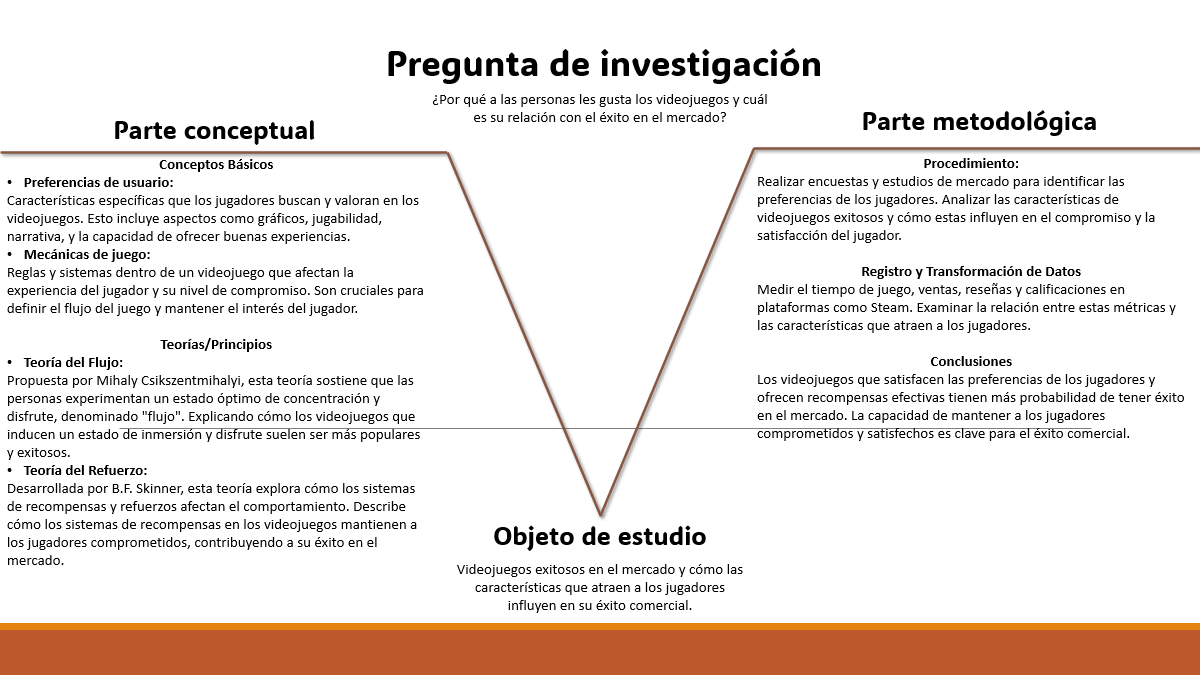
\includegraphics{imagenes/V-de-gowin.png}

}

\caption{Diagrama de Gowin}

\end{figure}%

Fuentes:

\begin{itemize}
\item
  Csikszentmihalyi (1990)
\item
  Skinner (1938)
\end{itemize}

\bookmarksetup{startatroot}

\chapter{Parte de escritura}\label{parte-de-escritura}

\section{Selección de la pregunta:}\label{selecciuxf3n-de-la-pregunta}

¿Por qué a las personas les atraen los videojuegos y cuál es su relación
con el éxito comercial de los videojuegos?

\subsection{Argumentación:}\label{argumentaciuxf3n}

La pregunta escogida tiene origen en la investigación realizada de las
otras tres preguntas potenciales. La razón principal es qué la misma
tiene la característica de englobar (no necesariamente en una magnitud
uniforrme) a las demás de manera explícita como ímplicita. Para
dilucidar la naturaleza de la pregunta, se mostrará la siguiente
comparación:

\textbf{(i)} ¿Qué características son fundamentales para el éxito
comercial de un videojuego dado el contexto donde fue publicado? ó ¿Por
qué a las personas les atraen los videojuegos y cuál es su relación con
el éxitocomercial de los videojuegos?

Primero, note que el corazón de la primera pregunta reside en las
palabras \emph{características} y \emph{fundamentales}. De esta
pregunta, podemos plantear las siguientes: ¿Existen características
generales que hagan que a las personas les gusten los videojuegos? y ¿Si
existen dichas características, qué tan fundamentales son en el mercado
de los videojuegos para la desición de los consumidores? Se puede
hallar, de manera parcial, una respuesta a ambas preguntas en el
escapismo que menciona Di Blasi (2019) en su respectivo artículo; pero
es que además esta respuesta funge de igual manera en la pregunta
elegida por el grupo. Finalmente, tras confrontar ambas preguntas y
notar esta relación: se determinó cuál pregunta resultó vencedora, o sea
la que se eligió.

\textbf{(ii)} ¿Por qué es importante analizar el mercado de los
videojuegos para reconocer desencadenantes del éxito de la industria? ó
¿Por qué a las personas les atraen los videojuegos y cuál es su relación
con el éxitocomercial de los videojuegos?

El vínculo entre estas dos preguntas no parece tan clara a primera
vista, no obstante y de manera empírica se pueden utilizar las
conclusiones del Estudio sobre juegos para móviles: hábitos en el sector
`gaming' (We Are Testers (2024)) para proponer respuestas a la primera
pregunta. En este estudio se mencionan dos cosas importantes:
\emph{frecuencia de juego} y \emph{celulares}, el celular es
posiblemente el objeto más utilizado del siglo ventiúno. ``El celular es
el objeto más utilizado'' es lo mismo que decir ``La frecuencia de uso
del celular corresponde a la mayor de otro objeto'', entonces es natural
pensar que si existen videojuegos de celulares, esto implicaría que no
es de extrañar que los videojuegos para móbiles sean tan populares; ¿Son
estas características fundamentales (relación con lo planteado en (i))
para el éxito de los videojuegos? Si la respuesta es afirmativa,
entonces por transitividad se llega a que esta podría ser una razón de
preferencia de los consumidores frente a los videojuegos. De semejante
manera se llega a la misma conclusión que en (i): la respuesta ante la
hipótesis planteada en este inciso funciona para ambas interrogantes.

\textbf{(iii)} ¿Cómo se puede analizar el mercado de los videojuegos? ó
¿Por qué a las personas les atraen los videojuegos y cuál es su relación
con el éxito comercial de los videojuegos?

Se desestimó fácilmente la primera pregunta, pues el mercado se puede
analizar desde las preferencias, y para entender las preferencias se
necesita entender el por qué de esta; o sea, el origen de la atracción
que los videojuegos han cultivado en millones de personas. \#

\bookmarksetup{startatroot}

\chapter{Bitácora 2}\label{bituxe1cora-2}

\bookmarksetup{startatroot}

\chapter{Parte de Planificación}\label{parte-de-planificaciuxf3n}

\section{Ordenamiento de la
Literatura}\label{ordenamiento-de-la-literatura}

\bookmarksetup{startatroot}

\chapter{Enlaces de la Literatura}\label{enlaces-de-la-literatura}

En su obra ``The Behavior of Organisms'' (1938), B.F. Skinner plantea
que el comportamiento se regula mediante un proceso de selección por
consecuencias, centrado en la interacción estímulo-respuesta. Su enfoque
analiza cómo los organismos cambian su conducta por los resultados
obtenidos de sus acciones. Por otra parte, este planteamiento contrasta
con la teoría de Csikszentmihalyi (1990), ya que él propone que el
comportamiento no depende de las consecuencias inmediatas, sino también
del nivel de inmersión que se logra cuando hay un equilibrio entre los
desafíos y las habilidades. Mientras Skinner pone énfasis en respuestas
automáticas ante estímulos, Csikszentmihalyi examina estados de
conciencia elevados, como el ``flujo''. Además, la obra de Skinner
ofrece una base experimental sólida sobre cómo el refuerzo modifica el
comportamiento, y el enfoque de Csikszentmihalyi complementa este modelo
al destacar la importancia de la motivación intrínseca y el disfrute de
la actividad como factores clave.

En ``Flow: The Psychology of Optimal Experience'' (1990), Mihaly
Csikszentmihalyi desarrolla el concepto de ``flujo'', un estado mental
caracterizado por la plena concentración y disfrute de una actividad
cuando las habilidades de la persona se alinean con el nivel de desafío
de la tarea. El concepto de ``flujo'' guarda una conexión relevante con
los estudios de Deterding et al.~(2022) sobre los videojuegos, que
señalan que la incertidumbre es crucial para que los jugadores
disfruten. Por otro lado, ambos enfoques destacan la importancia de
mantener un equilibrio: en el caso del ``flujo'', entre habilidad y
desafío; y en los videojuegos, entre previsibilidad e incertidumbre. En
la industria de los videojuegos, mantener un equilibrio entre las
habilidades del jugador y el reto que ofrece el juego es esencial para
garantizar una experiencia satisfactoria y prolongada, esto con el fin
del que el jugador se sienta cómodo realizando los desafíos, pero no tan
cómodo como para que considere el juego demasiado fácil o absurdo.

¿El estudio ``Innovate or Game Over?'' (2022), de Handrich et al.,
analiza cómo la innovación en las mecánicas y la presentación de los
videojuegos impacta directamente su éxito en el mercado. Los autores
destacan que las innovaciones en la jugabilidad pueden mejorar el
rendimiento inicial de un juego. El argumento sobre la necesidad de
innovar en los videojuegos se alinea con el análisis de Deterding et
al., quienes subrayan la importancia de la incertidumbre y el
procesamiento predictivo en la experiencia del jugador. Sin embargo,
mientras Deterding et al.~se enfocan en aspectos psicológicos, Handrich
et al.~adoptan una perspectiva más comercial y destacando cómo la
innovación en los videojuegos es clave para su competitividad en el
mercado. Ambos estudios revelan que la innovación no solo es crucial en
el diseño y las mecánicas de juego, sino también en la manera en que los
jugadores experimentan a esos cambios. Mantener el equilibrio entre las
expectativas del mercado y la experiencia del jugador resulta vital para
asegurar el éxito de un videojuego a largo y corto plazo.

En el estudio ``Mastering Uncertainty: A Predictive Processing Account
of Enjoying Uncertain Success in Video Game Play'' (2022), exploran cómo
la incertidumbre puede influir en el disfrute de los videojuegos y se
analiza cómo los jugadores manejan la incertidumbre, a través del
procesamiento predictivo, lo cual mantiene su interés en el juego.
Deterding et al proponen que la incertidumbre es un elemento esencial
para garantizar una buena experiencia al jugador, además sugieren que
estos desarrollan expectativas sobre los resultados lo que les permite
navegar la incertidumbre de manera efectiva. Y se dice que la
incertidumbre, en lugar de disminuir la satisfacción, mantiene a los
jugadores comprometidos y motivados lo que mejora su inmersión en el
juego. Por otro lado, al entender el papel de la incertidumbre los
desarrolladores deben considerar mecánicas del juego que puedan provocar
respuestas cognitivas que fomenten el disfrute. Además, los diseñadores
pueden crear experiencias más dinámicas que se adapten a las
expectativas cambiantes de los jugadores.

``The Impact of Video Games on the Players Behaviors: A Survey'' (2019)
de Quwaider, et al., es un estudio que per sé contrasta los efectos
negativos y positivos de los videojuegos tratando de hacerlo desde una
óptica generalizada. En este estudio, los autores mencionan aspectos
negativos de los videojuegos como: adicción a los videojuegos y recaídas
y conductas violentas. Este último aspecto se alinea con lo encontrado
por Di Blasi(2020) en su análisis sobre los juegos MMROPG; género
también mencionado en este estudio. De forma más general, se menciona
que los videojuegos de carácter competitivo son los gatilleros de este
tipo de conductas antisociales, lo cual tiene mucho sentido si se
compara con los eventos deportivos más importantes en el país; como lo
es alguna final entre equipos de primera división, cuyos fanáticos son
capaces de violentarse entre sí dado que su equipo perdió (ganó).

Un estudio que es clave para entender el mercado en la actualidad es el
de los sPorts o deportes electrónicos. Gracias al aporte de Sergio
Mesonero (2019) en su artículo ``eSports: pasado y presente de las
competiciones de videojuegos'', se puede llegar a incluso simpatizar con
lo que representa esta industria. No es muy difícil notar en redes
sociales como muchas personas están en contra del financiamiento que se
les da a las competencias electrónicas, y no es de extrañar pues la
sociedad está acostumbrada a presenciar competiciones donde el contacto
físico es clave. La simpatía puede venir de parte del reconocimiento que
se le hace a los competidores, quienes tienen que entrenar de manera
frecuente sus artificios videojueguiles. No es difícil notar que este
fenómeno involucra un sistema de recompensa basado en la incertidumbre,
(características evocadas en el estudio ``Mastering Uncertainty: A
Predictive Processing Account of Enjoying Uncertain Success in Video
Game Play'' (2022)) en donde las consecuencias de la misma son más
severas (se gana o incluso se pierde dinero).

``Unravelling the complexity of the Video Game Industry: An integrative
framework and future research directions'' (2023) es un estudio cuyo
enfoque es el mercado de los videojuegos desde un punto mucho más
económico. Los autores argumentaron las dimensiones monetarias que
abarca esta industria comprendida en millones de dólares. Los números
son buenos indicadores para argumentar la existencia de mercados
derivados de los videojuegos, como los son los sPorts mencionados por
Sergio Mesonero(2019) en su artículo ``eSports: pasado y presente de las
competiciones de videojuegos''. De acuerdo a Goh Edward et al., el
mercado de los videojuegos se mantendrá fuerte y se espera que siga
creciendo. Según la hipótesis del crecimiento en este mercado, los
jugadores esperarían juegos de calidad superior y más ideas innovadoras
como lo puede ser la creación de una nueva consola de sobremesa.

\bookmarksetup{startatroot}

\chapter{Análisis Estadísticos}\label{anuxe1lisis-estaduxedsticos}

\section{Análisis Descriptivo}\label{anuxe1lisis-descriptivo}

El resumen de cada variable constará de: la mediana, el promedio, mínimo
y máximo, rango y desviación estándar. Existirán variables como la fecha
de lanzamiento en donde se omitirán algunas mediciones.

\subsection{Resúmenes:}\label{resuxfamenes}

\begin{tcolorbox}[enhanced jigsaw, toprule=.15mm, rightrule=.15mm, colframe=quarto-callout-color-frame, colback=white, left=2mm, breakable, arc=.35mm, opacityback=0, bottomrule=.15mm, leftrule=.75mm]

\textbf{Jugadores estimados}:

\begin{itemize}
\item
  Mediana: 150 000.
\item
  Promedio: 861937,2.
\item
  Mínimo: 10000.
\item
  Máximo: 150000000.
\item
  Rango: 149999000.
\item
  Desviación estándar: 4003982,9.
\end{itemize}

\end{tcolorbox}

\begin{tcolorbox}[enhanced jigsaw, toprule=.15mm, rightrule=.15mm, colframe=quarto-callout-color-frame, colback=white, left=2mm, breakable, arc=.35mm, opacityback=0, bottomrule=.15mm, leftrule=.75mm]

\textbf{Precio de los videojuegos (en dólares)}:

\begin{itemize}
\item
  Mediana: 12,99.
\item
  Promedio: 15,03278
\item
  Mínimo: 0.
\item
  Máximo: 69,99.
\item
  Rango: 69,99.
\item
  Desviación estándar: 11,78411.
\end{itemize}

\end{tcolorbox}

\begin{tcolorbox}[enhanced jigsaw, toprule=.15mm, rightrule=.15mm, colframe=quarto-callout-color-frame, colback=white, left=2mm, breakable, arc=.35mm, opacityback=0, bottomrule=.15mm, leftrule=.75mm]

\textbf{Nota de Metacritic}:

\begin{itemize}
\item
  Mediana: 74.
\item
  Promedio: 72,93191.
\item
  Mínimo: 20.
\item
  Máximo: 97.
\item
  Rango: 77.
\item
  Desviación estándar: 10,58026.
\end{itemize}

\end{tcolorbox}

\begin{tcolorbox}[enhanced jigsaw, toprule=.15mm, rightrule=.15mm, colframe=quarto-callout-color-frame, colback=white, left=2mm, breakable, arc=.35mm, opacityback=0, bottomrule=.15mm, leftrule=.75mm]

\textbf{Reseñas positivas (positive)}:

\begin{itemize}
\item
  Mediana: 929.
\item
  Promedio: 12588,49.
\item
  Mínimo: 0.
\item
  Máximo: 5764420.
\item
  Rango: 5764420.
\item
  Desviación estándar: 106383,23.
\end{itemize}

\end{tcolorbox}

\begin{tcolorbox}[enhanced jigsaw, toprule=.15mm, rightrule=.15mm, colframe=quarto-callout-color-frame, colback=white, left=2mm, breakable, arc=.35mm, opacityback=0, bottomrule=.15mm, leftrule=.75mm]

\textbf{Negative (reseñas negativas)}:

\begin{itemize}
\item
  Mediana: 198.
\item
  Promedio: 1691,981.
\item
  Mínimo: 0.
\item
  Máximo: 766677.
\item
  Rango: 766677.
\item
  Desviación estándar: 14692,469.
\end{itemize}

\end{tcolorbox}

\begin{tcolorbox}[enhanced jigsaw, toprule=.15mm, rightrule=.15mm, colframe=quarto-callout-color-frame, colback=white, left=2mm, breakable, arc=.35mm, opacityback=0, bottomrule=.15mm, leftrule=.75mm]

\textbf{Fechas de lanzamiento}:

\begin{itemize}
\item
  Mínimo: 1997.
\item
  Máximo: 2024.
\item
  Rango: 27.\\
\end{itemize}

\end{tcolorbox}

\section{Propuesta Metodológica}\label{propuesta-metodoluxf3gica}

\subsection{Nuevos Métodos}\label{nuevos-muxe9todos}

Se formularán varios métodos que permitirán analizar el \textbf{Steam
Games Dataset} y predecir el éxito de los videojuegos en función de
variables clave:

\subsection{Análisis Exploratorio de Datos
(EDA)}\label{anuxe1lisis-exploratorio-de-datos-eda}

\textbf{Objetivo}: Obtener una comprensión inicial del dataset,
identificando patrones, anomalías y relaciones entre variables.

\textbf{Variables a analizar}:

- \textbf{Price}: Precio del videojuego.

- \textbf{Positive}: Número de reseñas positivas.

- \textbf{Negative}: Número de reseñas negativas.

- \textbf{User score}: Calificación otorgada por los usuarios.

- \textbf{Metacritic score}: Calificación del videojuego en Metacritic.

- \textbf{Estimated players}: Número estimado de propietarios/jugadores
del videojuego.

- \textbf{Release Date}: Fecha de lanzamiento del videojuego.

\textbf{Fuente}: Wickham y Grolemund (2017)

\subsection{Regresión Lineal
Múltiple}\label{regresiuxf3n-lineal-muxfaltiple}

\textbf{Objetivo}: Predecir el número estimado de propietarios de un
videojuego (\texttt{Estimated\ owners}) utilizando diversas variables
numéricas.

\textbf{Ecuación del Modelo}: \[
\text{Estimated owners} = \beta_0 + \beta_1 (\text{User score}) + \beta_2 (\text{Price}) + \beta_3 (\text{Positive}) + \epsilon
\] - \((\beta_0)\)\textbf{: Intercepto del modelo.}

\textbf{-} \((\beta_1, \beta_2, \beta_3)\): Coeficientes de las
variables predictoras.

\textbf{Descripción de las Variables}:

- \textbf{\texttt{User\ score}}: Calificación otorgada por los usuarios,
que puede influir en la popularidad del videojuego.

\begin{itemize}
\tightlist
\item
  \textbf{\texttt{Price}}: Precio del videojuego, que puede afectar su
  accesibilidad y, en consecuencia, el número de propietarios.
\end{itemize}

- \textbf{\texttt{Positive}}: Número de reseñas positivas, un indicador
que refleja la aceptación del juego por parte de la comunidad.

El modelo de regresión lineal múltiple proporciona una herramienta
poderosa para comprender cómo estas variables interactúan y afectan el
número estimado de propietarios de un videojuego.

\textbf{Fuente}: James et~al. (2021)

\subsection{Algoritmo de Clustering
(K-means)}\label{algoritmo-de-clustering-k-means}

\textbf{Objetivo}: Agrupar videojuegos en función de características
como \textbf{precio}, \textbf{reseñas positivas}, y
\textbf{calificación}. El algoritmo K-means identifica patrones en los
datos, permitiendo segmentar el mercado de videojuegos.

\textbf{Descripción del Método}:\\
K-means es un método de agrupamiento que divide un conjunto de datos en
(k) grupos basados en las características de los videojuegos. El proceso
incluye:

\begin{enumerate}
\def\labelenumi{\arabic{enumi}.}
\item
  \textbf{Inicialización}: Seleccionar (k) centroides iniciales
  aleatorios.
\item
  \textbf{Asignación}: Cada videojuego se asigna al clúster cuyo
  centroide está más cercano.
\item
  \textbf{Recalculación}: Se actualizan los centroides como el promedio
  de los puntos en cada clúster.
\item
  \textbf{Iteración}: Se repiten los pasos 2 y 3 hasta que los
  centroides se estabilizan.
\end{enumerate}

\textbf{Ecuación del Algoritmo}:\[
\text{Minimizar} \sum_{i=1}^{n} \sum_{j=1}^{k} \|x_i - c_j\|^2
\]

Donde \((x_i)\) es un videojuego y \((c_j)\) es el centroide del clúster
(j).

\textbf{Fuente}: MacQueen (1967)

\section*{Construcción de Fichas de
Resultados}\label{construcciuxf3n-de-fichas-de-resultados}
\addcontentsline{toc}{section}{Construcción de Fichas de Resultados}

\phantomsection\label{refs}
\begin{CSLReferences}{1}{0}
\bibitem[\citeproctext]{ref-Ref9}
Csikszentmihalyi, Mihaly. 1990. \emph{Flow: The Psychology of Optimal
Experience}. Harper \& Row.

\bibitem[\citeproctext]{ref-Ref5}
Desconocido, Autor. 2024a. {«Análisis de la industria del videojuego en
España»}. \emph{Riunet}.
\url{https://riunet.upv.es/bitstream/handle/10251/45702/Trabajo\%20final\%20carrera.pdf}.

\bibitem[\citeproctext]{ref-Ref6}
---------. 2024b. {«Plan de marketing para una empresa de videojuegos»}.
\emph{Universidad Nacional de Cuyo}.
\url{https://bdigital.uncu.edu.ar/objetos_digitales/15654/plan-de-marketing-para-una-empresa-de-videojuegos.pdf}.

\bibitem[\citeproctext]{ref-Ref8}
Deterding, Sebastian, Marc Malmdorf Andersen, Julian Kiverstein, y Mark
Miller. 2022. {«Mastering uncertainty: A predictive processing account
of enjoying uncertain success in video game play»}. \emph{Frontiers in
Psychology} 13.
\url{https://www.frontiersin.org/journals/psychology/articles/10.3389/fpsyg.2022.924953/full}.

\bibitem[\citeproctext]{ref-Ref2}
Di Blasi, Maria. 2019. {«Problematic video game use as an emotional
coping strategy: Evidence from a sample of MMORPG gamers»}.
\emph{Journal of Behavioral Addictions} 8 (1): 25-34.
https://doi.org/\url{https://doi.org/10.1556/2006.8.2019.02}.

\bibitem[\citeproctext]{ref-Ref3}
Guerrero Pastor, Marta. 2018. {«¿Qué hace divertido un videojuego?
Acercamiento al concepto de diversión a través del análisis de
videojuegos»}.
\url{https://rua.ua.es/dspace/bitstream/10045/73641/1/Que_hace_divertido_un_videojuego_Acercamiento_al_conce_GUERRERO_PASTOR_MARTA.pdf}.

\bibitem[\citeproctext]{ref-Ref7}
Handrich, Franziska, Sven Heidenreich, y Tobias Kraemer. 2022.
{«Innovate or game over? Examining effects of product innovativeness on
video game success»}. \emph{Electronic Markets} 32 (2).
\url{https://doi.org/10.1007/s12525-022-00521-7}.

\bibitem[\citeproctext]{ref-Ref1}
Hevia, Carme Mangiron i. 2012. {«Manga, anime y videojuegos japoneses:
análisis de los principales factores de su éxito global»}. \emph{Puertas
a la lectura}, n.º 24: 28-43.

\bibitem[\citeproctext]{ref-Ref15}
James, Gareth, Daniela Witten, Trevor Hastie, y Robert Tibshirani. 2021.
\emph{An Introduction to Statistical Learning with Applications in R}.
Springer. \url{https://www.statlearning.com}.

\bibitem[\citeproctext]{ref-Ref16}
MacQueen, J. 1967. {«Some Methods for Classification and Analysis of
Multivariate Observations»}. \emph{Proceedings of the Fifth Berkeley
Symposium on Mathematical Statistics and Probability} 1: 281-97.
\url{https://projecteuclid.org/euclid.bsmsp/1200512992}.

\bibitem[\citeproctext]{ref-Ref10}
Skinner, B. F. 1938. \emph{The Behavior of Organisms: An Experimental
Analysis}. Appleton-Century.

\bibitem[\citeproctext]{ref-Ref4}
STEAM, ON. s.~f. {«LA POLÍTICA A LA QUE JUGAMOS. CULTURA, VIDEOJUEGOS Y
LUDOFICCIÓN POLÍTICA EN LA PLATAFORMA STEAM»}.

\bibitem[\citeproctext]{ref-Ref13}
We Are Testers. 2024. {«Estudio de mercado sobre juegos para móviles y
gaming»}.
\url{https://www.wearetesters.com/estudios-de-mercado/gaming/}.

\bibitem[\citeproctext]{ref-Ref14}
Wickham, Hadley, y Garrett Grolemund. 2017. \emph{R for Data Science:
Import, Tidy, Transform, Visualize, and Model Data}. O'Reilly Media.
\url{https://r4ds.had.co.nz}.

\bibitem[\citeproctext]{ref-Ref12}
Wikipedia. 2024a. {«Video game mechanics»}.
\url{https://en.wikipedia.org/wiki/Video_game_mechanics}.

\bibitem[\citeproctext]{ref-Ref11}
---------. 2024b. {«Video game preferences»}.
\url{https://en.wikipedia.org/wiki/Video_game_preferences}.

\end{CSLReferences}



\end{document}
